\subsection{Bildegjenkjenning}

\subsection{Mekanisk Instalasjon}
Når flyet skal svinge er flyet avhenigig av å gjøre en roll.
Dette fører til at buken til flyet ikke lengre peker rett ned mot bakken.
Et kamera i en låst posisjon, vil i denne situasjonen kunne oppleve at
objektet det skulle ha i bildet forsvinner ut av bildekanten.
Ved å feste kameraet til en mekanisk rigg som kan kompensesere for at flyet beveger
seg vil dette problemet kunne løses.

For å beskytte kameraet ble det bestemt at kameraet skal kunne
trekkes inn i flyet ved landing.
Siden målene på fullskala fly ikke er fremstilt fra Kongsberg ble det
bestemt å følge målene på modellen i presentasjonen sendt fra Kongsberg.
Denne viser at plassen inne i er maksimalt 10.5 cm i høyden og 7.2 cm i bredden.
Kravet for riggen ble dermed at den ikke kunne oppta større plass i bredde
og høyde enn dette med kameraet tilfestet.
Det ble antatt at det for modellens skyld kunne brukes et lite kamera,
på størrelse med et mobilkamera. Den andre grunnen til å bygge en liten rigg
er for å hindre at vekten blir for stor.
Kameraet må ha mulighet til å bevege synsretningen i x- og y-retning, noe som krever to servoer. Itilleg trengs en ekstra servomotor for å kunne trekke kameraet inn i flyet ved landing.

\subsubsection{Servomotor}
En servomotor er en inretning som kan rotere en arm til en bestemt vinkelposisjon og holde posisjonen.
Det finnes mange forskjellige servomotorer, med forskjellige egenskaper i forhold til nøyaktighet, kraft, pris, størrelse, vekt, kontrollsignaler, motortyper og kildespenning. 
Enkle servomotorer kan bestå av enkle DC motorer med børster og kan bare justere posisjons mellom -90 til +90 grader fra senter, mens avanserte servoer kan ha børsteløse motorer og ha mulighet til full rotasjon, med kontrollbar vinkelhastighet og tilbakemelid av posisjon og fart. 
En servomotor er bygget opp av en elektrisk motor, en vinkelsensor og en kontroll enhet.
Et kommandosignal, som representere en vinkelposisjon, påtrykkes inngangen, dette fører til at motoren roterer i retning av denne posisjonen. Vinkelsensoren registrer hele tiden posisjonen til armen og kontrollenheten sammenlikner denne med den ønskede posisjonen. Når den ønskede vinkelposisjonen er nådd stopper motoren. Hvis armen skyves bort fra denne posisjonen vil kontrollenheten registere at den nåværende vinkelen avviker fra ønsket vinkel og motoren vil flytte armen tilbake i rett posisjon.

I dette prosjektet ble det brukt servomotorer av typen HD-1600A fra PowerHD [\ref{ref:PowerHD}]. Dette er en enkel analog servomotor, beregnet for radiostyrte modellfly, som består av en DC motor, en potensiometer som vinkelsensor og en kontrollenhet av typen YT2462B. For å kontrollere denne typen servomotorer brukes puls-bredde-modulasjon (PWM). I PWM sendes firkantpulser hvor pulslengden varieres, mens grunnfrekvensen holdes konstant. Informasjonen ligger dermed i lengden av pulsen. For styring av analoge RC servoer som HD-1600A er det vanlig å bruke en grunnfrekvens på 50Hz og bulsbredde på 1ms til 2ms [\ref{ref:SerCtrl}]. Figur \ref{fig:PWM} viser hvordan servovinkel avhenger av pulsbredde.

\begin{figure}[H]
\centering
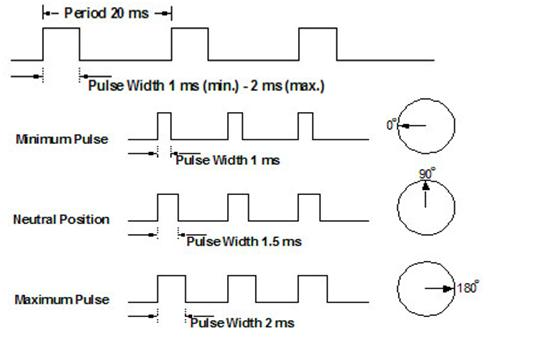
\includegraphics[width=0.8\textwidth]{img/pwm_servo.jpg}
\caption{PWM servo kontrollsignal}
\label{fig:PWM}
\end{figure}   
